% !TEX program = xelatex
\documentclass[aspectratio=169,11pt]{beamer}

\usetheme{AnnArbor}
\usecolortheme{beaver}
\setbeamertemplate{navigation symbols}{}
\setbeamertemplate{footline}[frame number]

\usepackage{fontspec}
\usepackage[vietnamese]{babel}
\setsansfont{DejaVu Sans}
\setmonofont{DejaVu Sans Mono}

\usepackage{graphicx}
\usepackage{booktabs}
\usepackage{array}
\usepackage{listings}
\usepackage{xcolor}
\usepackage{tikz}
\usetikzlibrary{positioning}

\graphicspath{{seaborn_ann_arbor_assets_v1/}}

\definecolor{codebg}{RGB}{248,248,248}
\definecolor{codeborder}{RGB}{220,220,220}
\definecolor{pyblue}{RGB}{0,80,150}
\definecolor{pygreen}{RGB}{40,120,70}
\definecolor{pygray}{RGB}{90,90,90}

\lstdefinestyle{pythonstyle}{
    language=Python,
    basicstyle=\ttfamily\scriptsize,
    keywordstyle=\color{pyblue}\bfseries,
    stringstyle=\color{pygreen},
    commentstyle=\color{pygray}\itshape,
    showstringspaces=false,
    breaklines=true,
    breakatwhitespace=true,
    frame=single,
    rulecolor=\color{codeborder},
    backgroundcolor=\color{codebg},
    tabsize=4,
    columns=fullflexible
}
\lstset{style=pythonstyle}

\title[Seaborn trong Python]{Giới thiệu Seaborn trong Python}
\subtitle{Trực quan hóa thống kê cho Data Science, Business và Economics}
\author{Duc-Minh Vu}
\institute{SLSCM Lab -- FDA -- NEU}
\date{\today}

\begin{document}

%------------------------------------------------
\begin{frame}
    \titlepage
\end{frame}

%------------------------------------------------
\begin{frame}{Mục tiêu học tập}
Sau bài này, người học có thể:
\begin{itemize}
    \item Giải thích Seaborn là gì và vì sao hữu ích trong phân tích dữ liệu.
    \item Phân biệt các nhóm biểu đồ chính: relational, categorical, distribution, regression, matrix và multi-plot grids.
    \item Vẽ các biểu đồ cơ bản: \texttt{lineplot}, \texttt{scatterplot}, \texttt{barplot}, \texttt{boxplot}, \texttt{histplot}, \texttt{heatmap}, \texttt{pairplot}.
    \item Dùng biến phân nhóm bằng \texttt{hue}, \texttt{style}, \texttt{size}, \texttt{row}, \texttt{col}.
    \item Diễn giải biểu đồ theo ngữ cảnh Data Science, Business và Economics.
\end{itemize}
\end{frame}

%------------------------------------------------
\begin{frame}{Seaborn là gì?}
\begin{columns}[T,onlytextwidth]
\column{0.52\textwidth}
\begin{itemize}
    \item Seaborn là thư viện Python để tạo \textbf{statistical visualizations}.
    \item Được xây dựng trên nền \textbf{Matplotlib}.
    \item Tích hợp tốt với \textbf{pandas DataFrame}.
    \item Có style và color palette đẹp hơn mặc định của Matplotlib.
    \item Phù hợp cho bước \textbf{Exploratory Data Analysis - EDA}.
\end{itemize}

\column{0.43\textwidth}
\begin{block}{Ý tưởng cốt lõi}
Thay vì tự xử lý quá nhiều chi tiết hình học, ta mô tả dữ liệu bằng:
\begin{center}
\texttt{x, y, data, hue, row, col}
\end{center}
Seaborn tự lo phần trình bày thống kê.
\end{block}
\end{columns}
\end{frame}

%------------------------------------------------
\begin{frame}{Seaborn nằm ở đâu trong hệ sinh thái Python?}
\begin{center}
\begin{tikzpicture}[node distance=0.9cm, every node/.style={font=\small}]
\node[draw, rounded corners, fill=blue!8, minimum width=3.7cm, minimum height=0.8cm] (pandas) {pandas: dữ liệu dạng bảng};
\node[draw, rounded corners, fill=green!8, below=of pandas, minimum width=3.7cm, minimum height=0.8cm] (seaborn) {Seaborn: biểu đồ thống kê};
\node[draw, rounded corners, fill=orange!10, below=of seaborn, minimum width=3.7cm, minimum height=0.8cm] (matplotlib) {Matplotlib: nền tảng vẽ};
\node[draw, rounded corners, fill=red!8, below=of matplotlib, minimum width=3.7cm, minimum height=0.8cm] (output) {Figure / Axes / PNG / PDF};
\draw[->, thick] (pandas) -- (seaborn);
\draw[->, thick] (seaborn) -- (matplotlib);
\draw[->, thick] (matplotlib) -- (output);
\end{tikzpicture}
\end{center}
\vspace{0.2cm}
\begin{alertblock}{Ghi nhớ}
Seaborn không thay thế Matplotlib hoàn toàn. Thường ta dùng Seaborn để vẽ nhanh, rồi dùng Matplotlib để chỉnh tiêu đề, nhãn trục, bố cục và lưu hình.
\end{alertblock}
\end{frame}

%------------------------------------------------
\begin{frame}[fragile]{Cài đặt và import}
\begin{columns}[T,onlytextwidth]
\column{0.48\textwidth}
\textbf{Cài đặt bằng pip}
\begin{lstlisting}
pip install seaborn
\end{lstlisting}

\textbf{Cài đặt bằng conda}
\begin{lstlisting}
conda install seaborn
\end{lstlisting}

\column{0.48\textwidth}
\textbf{Import thường dùng}
\begin{lstlisting}
import seaborn as sns
import matplotlib.pyplot as plt
import pandas as pd
import numpy as np
\end{lstlisting}

\begin{block}{Phụ thuộc chính}
Python, NumPy, SciPy, pandas và Matplotlib.
\end{block}
\end{columns}
\end{frame}

%------------------------------------------------
\begin{frame}{Các nhóm biểu đồ trong Seaborn}
\small
\begin{tabular}{p{0.22\textwidth}p{0.34\textwidth}p{0.31\textwidth}}
\toprule
\textbf{Nhóm} & \textbf{Mục tiêu} & \textbf{Ví dụ hàm} \\
\midrule
Relational plots & Quan hệ giữa hai biến & \texttt{lineplot}, \texttt{scatterplot} \\
Categorical plots & So sánh theo nhóm/loại & \texttt{barplot}, \texttt{boxplot}, \texttt{violinplot} \\
Distribution plots & Phân phối của biến & \texttt{histplot}, \texttt{kdeplot} \\
Regression plots & Quan hệ kèm đường hồi quy & \texttt{regplot}, \texttt{lmplot} \\
Matrix plots & Ma trận, tương quan & \texttt{heatmap} \\
Multi-plot grids & Nhiều biểu đồ theo nhóm & \texttt{FacetGrid}, \texttt{catplot}, \texttt{relplot} \\
\bottomrule
\end{tabular}
\vspace{0.3cm}
\begin{block}{Cách chọn nhanh}
Câu hỏi về xu hướng dùng lineplot; câu hỏi về tương quan dùng scatterplot; câu hỏi về phân phối dùng histplot/boxplot; câu hỏi về nhiều biến số dùng heatmap hoặc pairplot.
\end{block}
\end{frame}

%------------------------------------------------
\section{Relational plots}

\begin{frame}[fragile]{1. Lineplot - xu hướng theo thời gian}
\begin{columns}[T,onlytextwidth]
\column{0.46\textwidth}
\begin{lstlisting}
import seaborn as sns
import matplotlib.pyplot as plt

sns.lineplot(
    data=df,
    x="timepoint",
    y="signal",
    hue="region",
    marker="o"
)
plt.show()
\end{lstlisting}

\begin{itemize}
    \item Phù hợp với dữ liệu có thứ tự: thời gian, kỳ học, quý, năm.
    \item \texttt{hue} tách nhiều đường theo nhóm.
\end{itemize}

\column{0.50\textwidth}
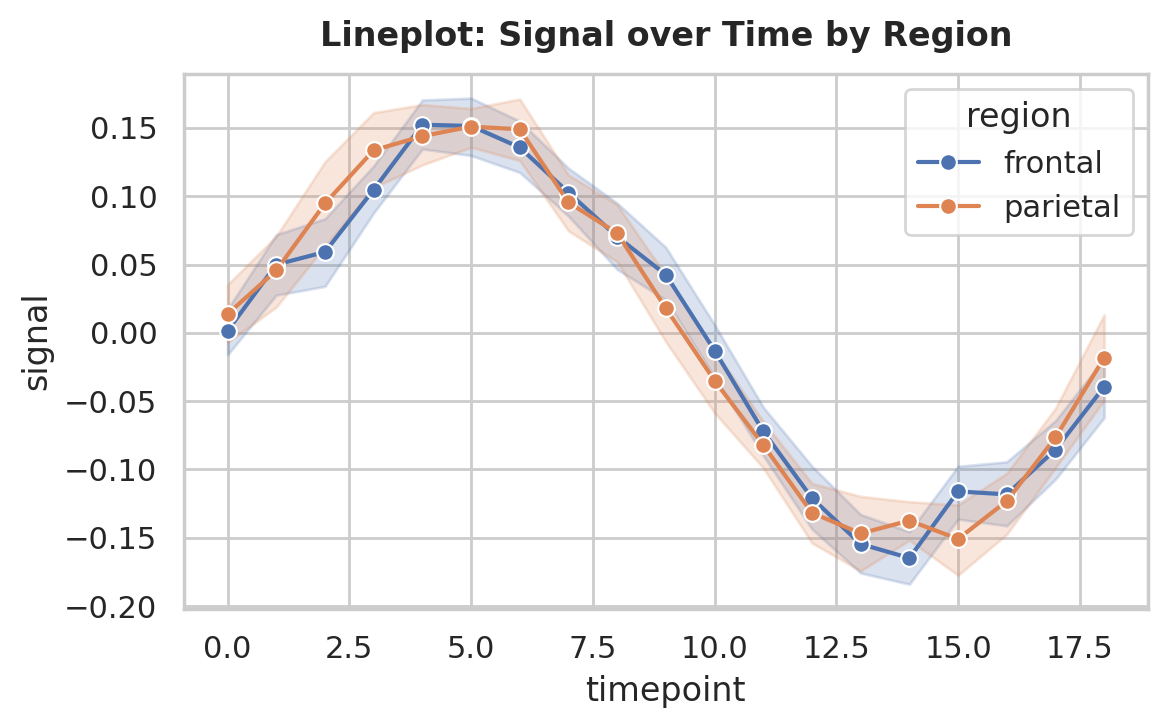
\includegraphics[width=\linewidth]{lineplot.png}
\end{columns}
\end{frame}

%------------------------------------------------
\begin{frame}{Ứng dụng Lineplot trong phân tích}
\begin{columns}[T,onlytextwidth]
\column{0.48\textwidth}
\textbf{Business}
\begin{itemize}
    \item Doanh thu theo tháng.
    \item Số đơn hàng theo kênh bán.
    \item Tỷ lệ chuyển đổi theo chiến dịch.
\end{itemize}

\column{0.48\textwidth}
\textbf{Economics}
\begin{itemize}
    \item Inflation theo quý.
    \item GDP growth theo năm.
    \item Unemployment rate theo thời gian.
\end{itemize}
\end{columns}

\vspace{0.3cm}
\begin{alertblock}{Câu hỏi phân tích}
Đường nào tăng nhanh nhất? Có điểm gãy xu hướng hay mùa vụ không? Có thời điểm bất thường cần giải thích không?
\end{alertblock}
\end{frame}

%------------------------------------------------
\begin{frame}[fragile]{2. Scatterplot - quan hệ giữa hai biến số}
\begin{columns}[T,onlytextwidth]
\column{0.46\textwidth}
\begin{lstlisting}
sns.scatterplot(
    data=df,
    x="total_bill",
    y="tip",
    hue="day"
)
plt.show()
\end{lstlisting}

\begin{itemize}
    \item Mỗi điểm là một quan sát.
    \item Dùng để xem quan hệ, cụm, ngoại lệ.
    \item \texttt{hue}, \texttt{size}, \texttt{style} giúp thêm biến phân nhóm.
\end{itemize}

\column{0.50\textwidth}
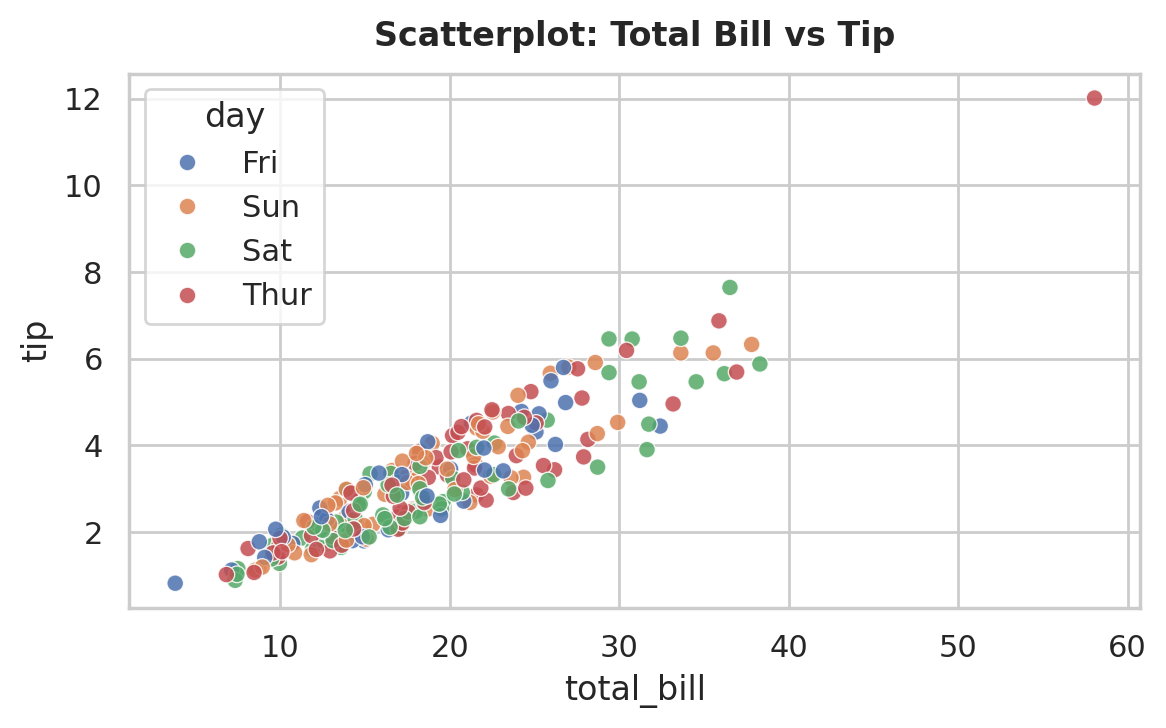
\includegraphics[width=\linewidth]{scatterplot.png}
\end{columns}
\end{frame}

%------------------------------------------------
\begin{frame}{Diễn giải Scatterplot}
\begin{block}{Khi đọc scatterplot, hãy hỏi}
\begin{itemize}
    \item Hai biến có cùng tăng/cùng giảm không?
    \item Quan hệ có tuyến tính hay phi tuyến?
    \item Có cụm dữ liệu khác nhau theo nhóm không?
    \item Có outlier nào đáng điều tra không?
\end{itemize}
\end{block}

\begin{exampleblock}{Ví dụ Data Science}
Trong bài toán churn, scatterplot giữa \texttt{Tenure} và \texttt{MonthlyCharge}, tô màu theo \texttt{Churn}, giúp xem nhóm rời bỏ có tập trung ở khách hàng mới hoặc chi phí cao hay không.
\end{exampleblock}
\end{frame}

%------------------------------------------------
\section{Categorical plots}

\begin{frame}[fragile]{3. Barplot - so sánh trung bình theo nhóm}
\begin{columns}[T,onlytextwidth]
\column{0.46\textwidth}
\begin{lstlisting}
sns.barplot(
    data=tips,
    x="day",
    y="total_bill"
)
plt.show()
\end{lstlisting}

\begin{itemize}
    \item So sánh giá trị số theo danh mục.
    \item Mặc định hiển thị trung bình.
    \item Có thể kèm khoảng tin cậy.
\end{itemize}

\column{0.50\textwidth}
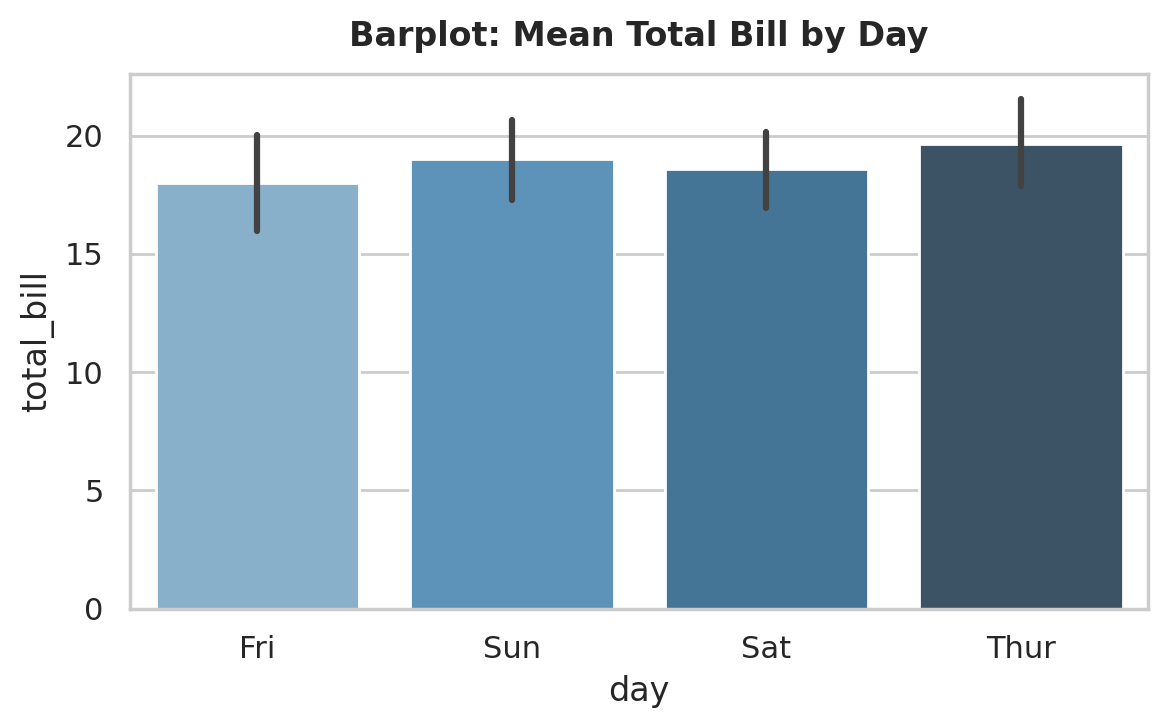
\includegraphics[width=\linewidth]{barplot.png}
\end{columns}
\end{frame}

%------------------------------------------------
\begin{frame}{Lưu ý khi dùng Barplot}
\begin{itemize}
    \item Barplot trong Seaborn thường biểu diễn \textbf{mean}, không phải tổng.
    \item Nếu cần tổng doanh thu theo khu vực, nên tổng hợp trước bằng pandas.
    \item Khoảng tin cậy giúp thấy mức độ bất định của ước lượng.
    \item Với dữ liệu lệch mạnh, chỉ nhìn trung bình có thể gây hiểu sai.
\end{itemize}

\begin{alertblock}{Sai lầm phổ biến}
Nhầm barplot của Seaborn với biểu đồ tổng. Cần đọc rõ: trục Y đang là mean, sum, count hay tỷ lệ?
\end{alertblock}
\end{frame}

%------------------------------------------------
\begin{frame}[fragile]{4. Boxplot - phân phối theo nhóm}
\begin{columns}[T,onlytextwidth]
\column{0.46\textwidth}
\begin{lstlisting}
sns.boxplot(
    data=tips,
    x="day",
    y="total_bill"
)
plt.show()
\end{lstlisting}

\begin{itemize}
    \item Thể hiện median, quartiles, spread và outliers.
    \item Hữu ích khi so sánh phân phối giữa các nhóm.
    \item Thường dùng trước khi modeling để phát hiện nhóm khác biệt.
\end{itemize}

\column{0.50\textwidth}
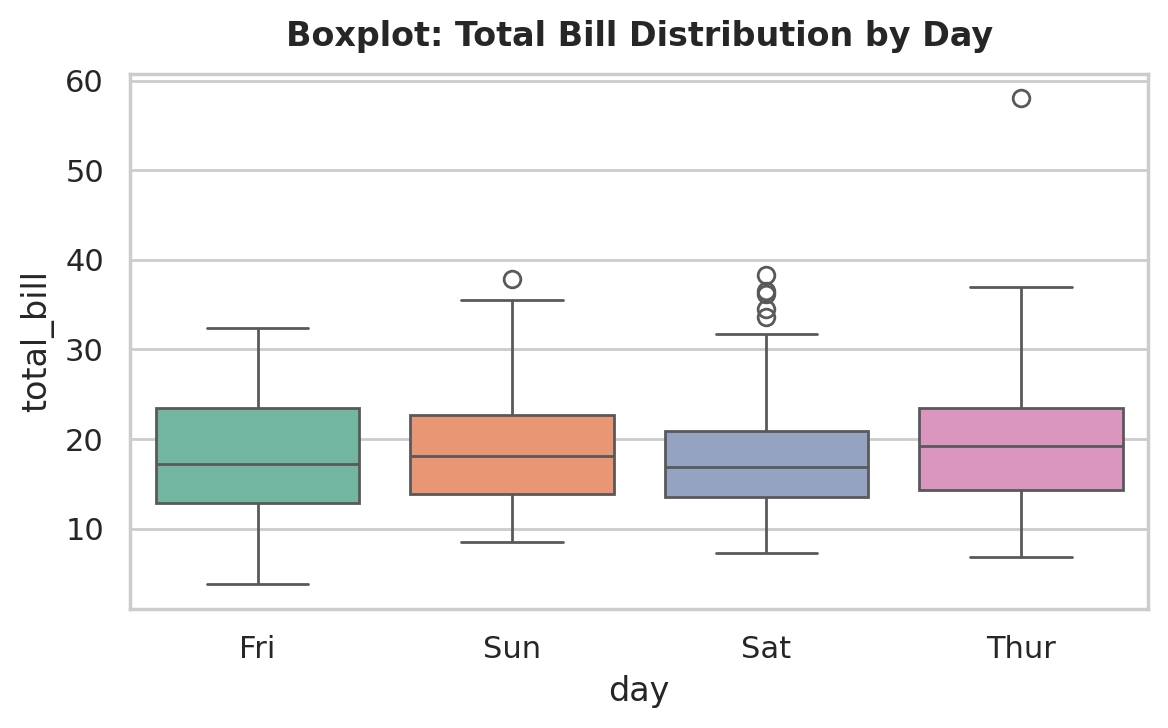
\includegraphics[width=\linewidth]{boxplot.png}
\end{columns}
\end{frame}

%------------------------------------------------
\begin{frame}{Boxplot trả lời câu hỏi gì?}
\begin{columns}[T,onlytextwidth]
\column{0.48\textwidth}
\textbf{Trong Business}
\begin{itemize}
    \item Nhóm khách hàng nào chi tiêu cao hơn?
    \item Kênh bán nào có biến động doanh thu lớn hơn?
    \item Có outlier bất thường không?
\end{itemize}

\column{0.48\textwidth}
\textbf{Trong Economics}
\begin{itemize}
    \item Tỉnh nào có thu nhập phân tán mạnh?
    \item Nhóm ngành nào có năng suất biến động lớn?
    \item Dữ liệu có lệch phải/lệch trái không?
\end{itemize}
\end{columns}
\end{frame}

%------------------------------------------------
\section{Distribution and matrix plots}

\begin{frame}[fragile]{5. Histplot - phân phối của một biến}
\begin{columns}[T,onlytextwidth]
\column{0.46\textwidth}
\begin{lstlisting}
sns.histplot(
    tips["total_bill"],
    kde=True
)
plt.show()
\end{lstlisting}

\begin{itemize}
    \item Dùng để xem biến tập trung ở đâu.
    \item \texttt{kde=True} thêm đường mật độ trơn.
    \item Hữu ích để phát hiện lệch phân phối và outliers.
\end{itemize}

\column{0.50\textwidth}
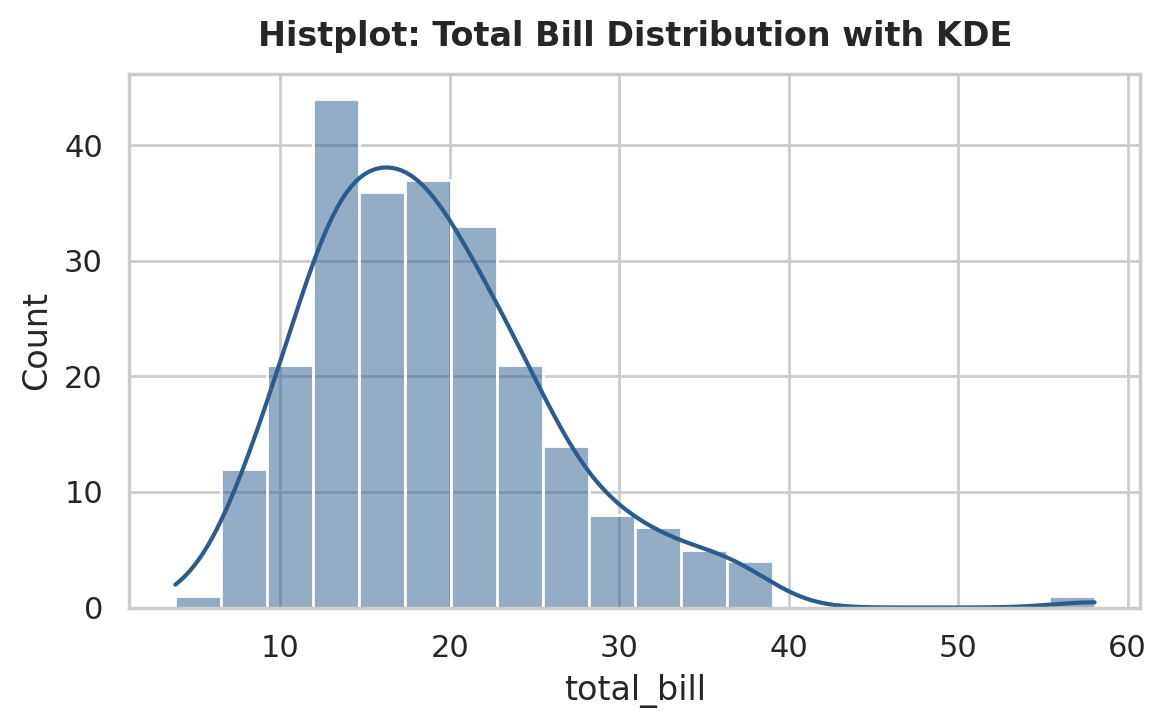
\includegraphics[width=\linewidth]{histplot.png}
\end{columns}
\end{frame}

%------------------------------------------------
\begin{frame}{Khi nào dùng Histplot?}
\begin{block}{Các câu hỏi phù hợp}
\begin{itemize}
    \item Thu nhập khách hàng tập trung quanh mức nào?
    \item Phần lớn đơn hàng có giá trị thấp hay cao?
    \item Biến có phân phối chuẩn không?
    \item Có cần log-transform trước khi modeling không?
\end{itemize}
\end{block}

\begin{exampleblock}{Gợi ý thực hành}
Với biến lệch phải như income, spending, order value, hãy thử vẽ thêm \texttt{np.log(x)} để kiểm tra phân phối sau biến đổi log.
\end{exampleblock}
\end{frame}

%------------------------------------------------
\begin{frame}[fragile]{6. Heatmap - ma trận tương quan}
\begin{columns}[T,onlytextwidth]
\column{0.46\textwidth}
\begin{lstlisting}
corr = df.corr(numeric_only=True)

sns.heatmap(
    corr,
    annot=True,
    cmap="coolwarm"
)
plt.show()
\end{lstlisting}

\begin{itemize}
    \item Dùng màu để biểu diễn giá trị trong ma trận.
    \item Rất phổ biến cho correlation matrix.
    \item Giúp phát hiện biến liên hệ mạnh hoặc đa cộng tuyến.
\end{itemize}

\column{0.50\textwidth}
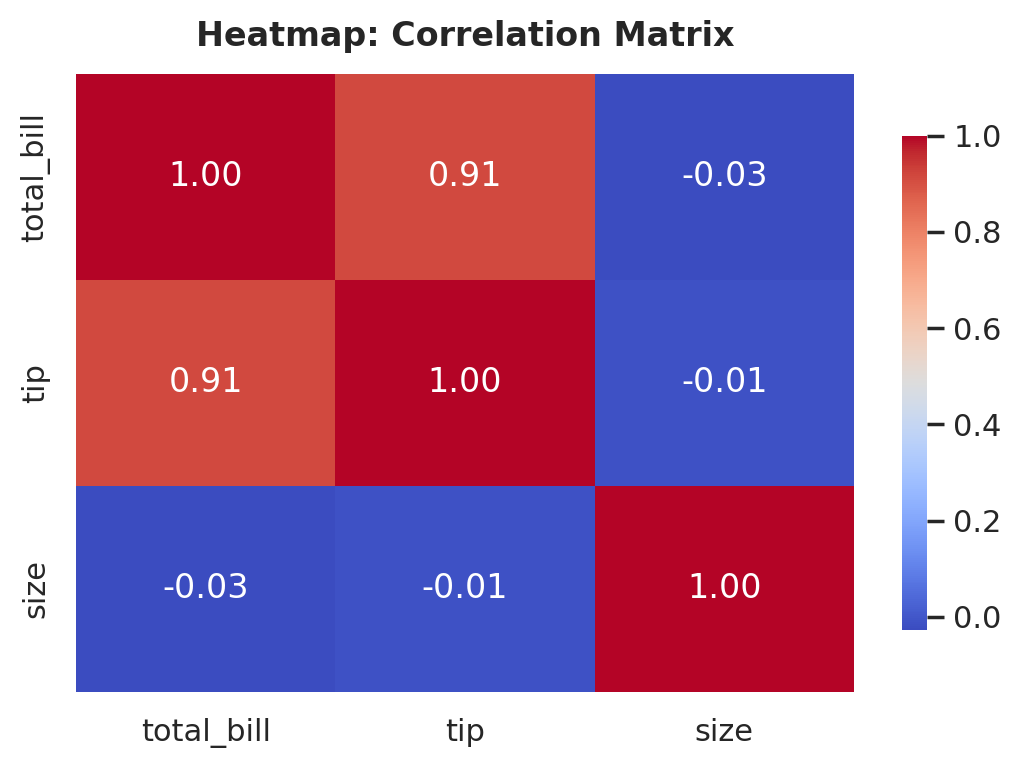
\includegraphics[width=\linewidth]{heatmap.png}
\end{columns}
\end{frame}

%------------------------------------------------
\begin{frame}{Diễn giải Heatmap cẩn thận}
\begin{itemize}
    \item Correlation gần 1: hai biến có xu hướng tăng cùng nhau.
    \item Correlation gần -1: một biến tăng, biến kia có xu hướng giảm.
    \item Correlation gần 0: không có quan hệ tuyến tính rõ ràng.
    \item Correlation không chứng minh quan hệ nhân quả.
\end{itemize}

\begin{alertblock}{Trong modeling}
Nếu hai biến đầu vào tương quan quá cao, mô hình tuyến tính có thể khó diễn giải. Khi đó cần xem xét feature selection, PCA hoặc regularization.
\end{alertblock}
\end{frame}

%------------------------------------------------
\section{Multi-variable EDA}

\begin{frame}[fragile]{7. Pairplot - quan hệ từng cặp biến}
\begin{columns}[T,onlytextwidth]
\column{0.42\textwidth}
\begin{lstlisting}
sns.pairplot(
    iris,
    hue="species"
)
plt.show()
\end{lstlisting}

\begin{itemize}
    \item Vẽ scatterplot cho từng cặp biến số.
    \item Đường chéo thường là phân phối của từng biến.
    \item Phù hợp để nhìn nhanh cấu trúc dữ liệu trước khi modeling.
\end{itemize}

\column{0.54\textwidth}
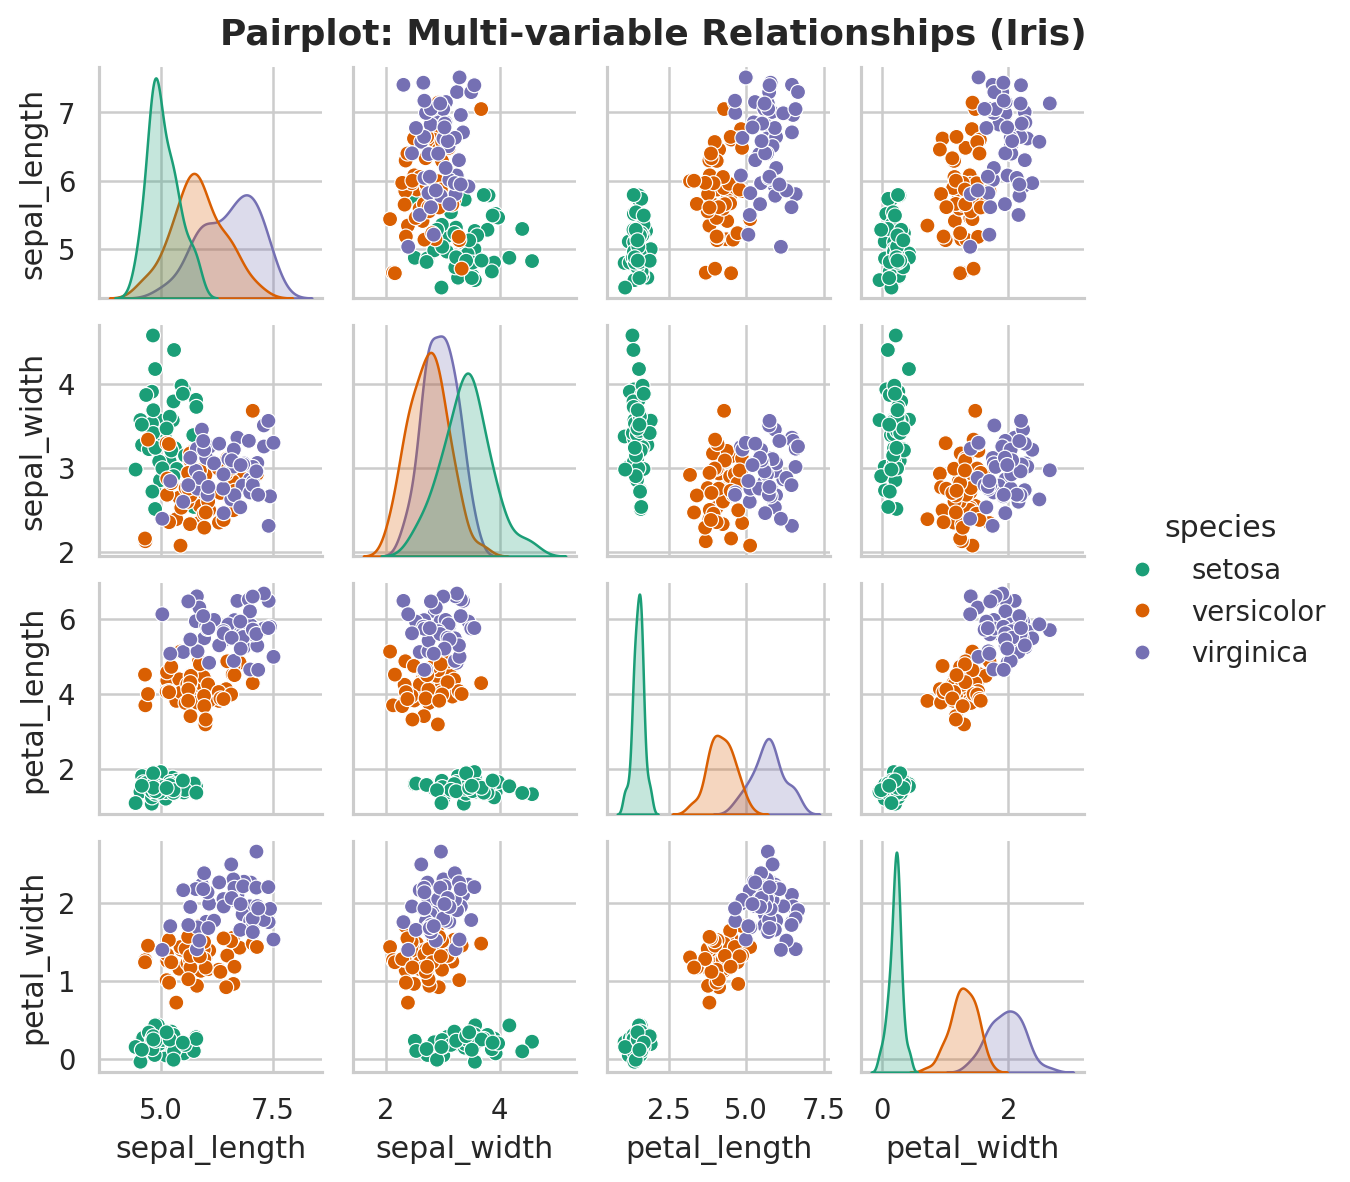
\includegraphics[width=\linewidth]{pairplot.png}
\end{columns}
\end{frame}

%------------------------------------------------
\begin{frame}[fragile]{FacetGrid - chia biểu đồ theo nhóm}
\begin{lstlisting}
g = sns.FacetGrid(
    data=df,
    row="region",
    col="product_type"
)
g.map_dataframe(
    sns.scatterplot,
    x="price",
    y="demand"
)
plt.show()
\end{lstlisting}

\begin{block}{Khi nào dùng FacetGrid?}
Khi biểu đồ quá rối vì có nhiều nhóm, thay vì nhồi tất cả vào một hình, ta chia thành nhiều ô nhỏ có cùng trục để so sánh dễ hơn.
\end{block}
\end{frame}

%------------------------------------------------
\begin{frame}{Seaborn và Matplotlib: dùng cùng nhau}
\begin{columns}[T,onlytextwidth]
\column{0.48\textwidth}
\textbf{Seaborn làm tốt}
\begin{itemize}
    \item Vẽ nhanh biểu đồ thống kê.
    \item Tự xử lý grouping/aggregation.
    \item Style đẹp, nhất quán.
    \item Dễ dùng với pandas.
\end{itemize}

\column{0.48\textwidth}
\textbf{Matplotlib làm tốt}
\begin{itemize}
    \item Chỉnh figure/axes chi tiết.
    \item Thêm annotation, đường tham chiếu.
    \item Tùy biến layout nhiều subplot.
    \item Lưu file chất lượng cao.
\end{itemize}
\end{columns}

\vspace{0.2cm}
\begin{center}
\textbf{Workflow tốt:} \texttt{sns.plot(..., ax=ax)} $\rightarrow$ \texttt{ax.set\_title(...)} $\rightarrow$ \texttt{fig.savefig(...)}
\end{center}
\end{frame}

%------------------------------------------------
\begin{frame}[fragile]{Workflow mẫu cho một biểu đồ chuyên nghiệp}
\begin{lstlisting}
fig, ax = plt.subplots(figsize=(8, 5))

sns.scatterplot(
    data=df,
    x="revenue",
    y="profit",
    hue="segment",
    alpha=0.7,
    ax=ax
)

ax.set_title("Revenue vs Profit by Segment")
ax.set_xlabel("Revenue")
ax.set_ylabel("Profit")
ax.legend(title="Segment")
plt.tight_layout()
plt.show()
\end{lstlisting}

\begin{block}{Thông điệp}
Seaborn tạo biểu đồ chính. Matplotlib hoàn thiện phần trình bày.
\end{block}
\end{frame}

%------------------------------------------------
\section{Ứng dụng và thực hành}

\begin{frame}{Ứng dụng trong Data Science}
\begin{itemize}
    \item \textbf{Trước modeling:} hiểu phân phối biến, outliers, missing patterns.
    \item \textbf{Feature engineering:} phát hiện biến cần log-transform hoặc chuẩn hóa.
    \item \textbf{Classification:} so sánh feature giữa các class bằng boxplot/histplot.
    \item \textbf{Regression:} kiểm tra quan hệ giữa predictor và target bằng scatterplot/regplot.
    \item \textbf{Model interpretation:} trực quan hóa residuals, errors, feature importance.
\end{itemize}
\end{frame}

%------------------------------------------------
\begin{frame}{Ứng dụng trong Business và Economics}
\begin{columns}[T,onlytextwidth]
\column{0.48\textwidth}
\textbf{Business Analytics}
\begin{itemize}
    \item Sales dashboard.
    \item Customer segmentation.
    \item Churn analysis.
    \item Pricing và demand analysis.
    \item Campaign performance.
\end{itemize}

\column{0.48\textwidth}
\textbf{Economics}
\begin{itemize}
    \item Inflation, GDP, unemployment.
    \item So sánh vùng/nhóm ngành.
    \item Phân phối thu nhập.
    \item Tương quan giữa chỉ số kinh tế.
    \item Visual storytelling cho báo cáo chính sách.
\end{itemize}
\end{columns}
\end{frame}

%------------------------------------------------
\begin{frame}{Nguyên tắc chọn biểu đồ}
\small
\begin{tabular}{p{0.34\textwidth}p{0.26\textwidth}p{0.30\textwidth}}
\toprule
\textbf{Câu hỏi} & \textbf{Biểu đồ nên dùng} & \textbf{Ví dụ} \\
\midrule
Xu hướng theo thời gian? & Lineplot & Doanh thu theo tháng \\
Hai biến liên hệ thế nào? & Scatterplot & Price và Demand \\
So sánh trung bình theo nhóm? & Barplot & AOV theo Region \\
Phân phối khác nhau giữa nhóm? & Boxplot/Violinplot & Income theo Segment \\
Một biến phân phối ra sao? & Histplot/KDE & Customer spending \\
Các biến số liên hệ với nhau? & Heatmap/Pairplot & Correlation matrix \\
\bottomrule
\end{tabular}
\end{frame}

%------------------------------------------------
\begin{frame}{Sai lầm thường gặp khi vẽ bằng Seaborn}
\begin{enumerate}
    \item Dùng biểu đồ đẹp nhưng không trả lời câu hỏi phân tích.
    \item Không biết trục Y đang là mean, count, sum hay tỷ lệ.
    \item Quá nhiều nhóm trong một biểu đồ làm hình rối.
    \item Không đặt title, xlabel, ylabel hoặc legend rõ ràng.
    \item Kết luận nhân quả chỉ từ correlation/scatterplot.
    \item Không kiểm tra outliers và phân phối trước khi modeling.
\end{enumerate}
\end{frame}

%------------------------------------------------
\begin{frame}{Bài tập lớn 1 - Customer Churn EDA}
\textbf{Bối cảnh:} Công ty subscription muốn hiểu vì sao khách hàng rời bỏ dịch vụ.

\vspace{0.2cm}
\textbf{Dữ liệu gợi ý:} \texttt{Tenure}, \texttt{MonthlyCharge}, \texttt{SupportCalls}, \texttt{Contract}, \texttt{Churn}.

\vspace{0.2cm}
\textbf{Yêu cầu trực quan hóa:}
\begin{itemize}
    \item Barplot/countplot cho phân phối \texttt{Churn}.
    \item Histplot \texttt{Tenure} theo \texttt{Churn}.
    \item Boxplot \texttt{MonthlyCharge} theo \texttt{Churn}.
    \item Scatterplot \texttt{Tenure} - \texttt{MonthlyCharge}, tô màu theo \texttt{Churn}.
\end{itemize}

\textbf{Đầu ra:} 3 insight và 2 đề xuất biến đầu vào cho mô hình churn.
\end{frame}

%------------------------------------------------
\begin{frame}{Bài tập lớn 2 - Business Sales Dashboard}
\textbf{Bối cảnh:} Chuỗi bán lẻ cần theo dõi doanh thu, lợi nhuận và khu vực bán hàng.

\vspace{0.2cm}
\textbf{Yêu cầu trực quan hóa:}
\begin{itemize}
    \item Lineplot doanh thu theo tháng, \texttt{hue=Region}.
    \item Barplot lợi nhuận trung bình theo nhóm sản phẩm.
    \item Boxplot order value theo kênh bán.
    \item Heatmap correlation giữa \texttt{Revenue}, \texttt{Profit}, \texttt{Discount}, \texttt{Orders}.
\end{itemize}

\textbf{Câu hỏi:}
\begin{itemize}
    \item Kênh/khu vực nào có performance tốt nhất?
    \item Discount có đi cùng profit thấp hơn không?
    \item Có nhóm nào doanh thu cao nhưng lợi nhuận thấp không?
\end{itemize}
\end{frame}

%------------------------------------------------
\begin{frame}{Bài tập lớn 3 - Economics Indicators}
\textbf{Bối cảnh:} Phân tích bộ chỉ số kinh tế theo quý.

\vspace{0.2cm}
\textbf{Biến gợi ý:} \texttt{Quarter}, \texttt{Inflation}, \texttt{Unemployment}, \texttt{GDPGrowth}, \texttt{InterestRate}.

\vspace{0.2cm}
\textbf{Yêu cầu trực quan hóa:}
\begin{itemize}
    \item Lineplot cho từng chỉ số theo thời gian.
    \item Scatterplot Inflation - Unemployment.
    \item Heatmap correlation giữa các chỉ số.
    \item FacetGrid để so sánh nhiều quốc gia/vùng nếu có.
\end{itemize}

\textbf{Đầu ra:} economic commentary 150-200 từ, nêu rõ điều gì có thể và không thể kết luận từ biểu đồ.
\end{frame}

%------------------------------------------------
\begin{frame}{Tổng kết}
\begin{itemize}
    \item Seaborn giúp trực quan hóa dữ liệu nhanh, đẹp và nhất quán hơn.
    \item Seaborn đặc biệt mạnh trong EDA vì làm việc trực tiếp với pandas DataFrame.
    \item Matplotlib vẫn cần thiết để tinh chỉnh biểu đồ và tạo layout chuyên nghiệp.
    \item Chọn biểu đồ phải bắt đầu từ câu hỏi phân tích, không bắt đầu từ hàm vẽ.
    \item Trong Data Science, Business và Economics, biểu đồ tốt phải hỗ trợ ra quyết định hoặc đặt câu hỏi tiếp theo.
\end{itemize}
\end{frame}

%------------------------------------------------
\begin{frame}{Câu hỏi ôn tập nhanh}
\begin{enumerate}
    \item Khi nào nên dùng \texttt{lineplot} thay vì \texttt{scatterplot}?
    \item \texttt{hue} trong Seaborn có tác dụng gì?
    \item Barplot của Seaborn mặc định biểu diễn tổng hay trung bình?
    \item Boxplot cho ta biết những thông tin nào về phân phối?
    \item Vì sao correlation heatmap không đủ để kết luận quan hệ nhân quả?
    \item Trong một EDA report, vì sao cần kết hợp nhiều loại biểu đồ?
\end{enumerate}
\end{frame}

\end{document}
